\section{Introduction}

\subsection{Abstract}
    Nowadays, a need to analyze more complex data arises.
    Some objects and relations can not be represented as vectors in Euclidean space, and, therefore, we have to consider graphs --- sets of nodes and connections between them --- as a subject of analysis.
    This poses a huge problem: we have to invent new algorithms, adapt known techniques and constantly improve them in order to work with such a complex data.
    Our goal is to research the efficiency of several tweaks of existing models. 
    
\subsection{Relevance}
    The field of research (graph neural networks) might be considered relatively new, and, therefore, there is a huge number of possible improvements to be made to existing models and approaches.
    Our ultimate goal is to improve the accuracy of node and graph classification.

    For example, one of the proposed changes is to modify a Laplacian in such a way that it does not break existing model and improves it.
    Our initial results have shown that our approach indeed works well on Karate club dataset, where we had to classify nodes:

    \begin{figure}[h]
        \centering
        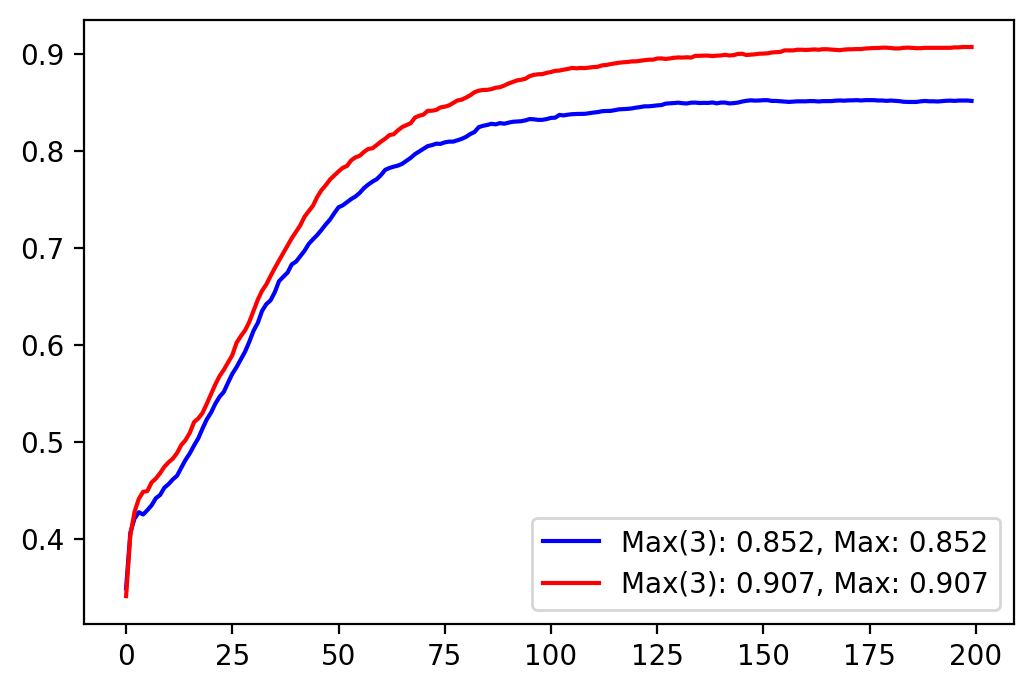
\includegraphics[width=0.6\textwidth]{custom_laplacian_accuracy.jpg}
        \caption{Default Laplacian (in blue) versus our Laplacian (in red). Y-axis is the accuracy, X-axis is the number of epochs}
    \end{figure}

\subsection{Subject of research}
    As we established, we want to consider several changes in order to improve the accuracy.
    The tweaks we propose include but are not limited to:
    \begin{itemize}
        \item \textit{Altering the way we compute Laplacian} --- a characteristic matrix of a graph.
        \item \textit{Edge embeddings}
        \item \textit{Using connectivity over simplices of higher dimension}. This means that in some cases we might want to consider a group of nodes as a separate object, therefore, increasing the connectivity factor. We will only work with 3-simplices:
            \begin{figure}[h]
                \begin{multicols}{2}
                    \centering
                    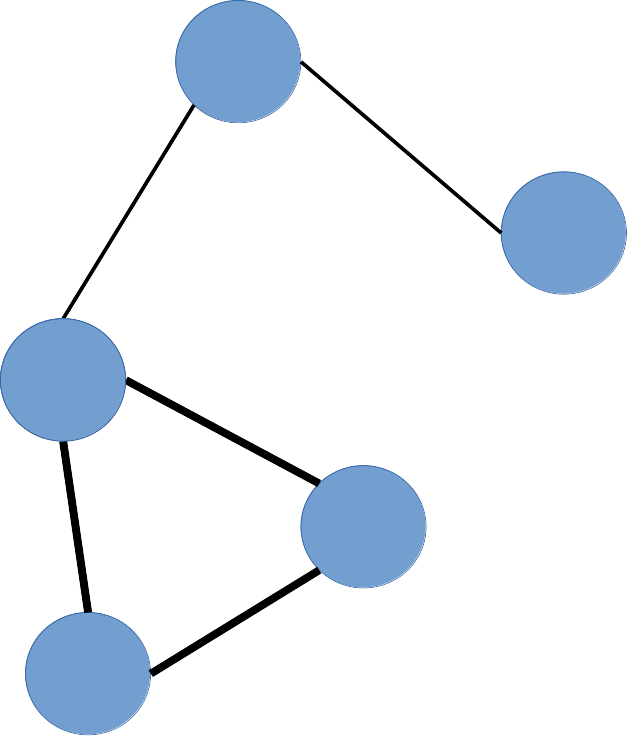
\includegraphics[width=0.2\textwidth]{simplex_1.png}
                    \caption{A part of some graph}
        
                    \centering
                    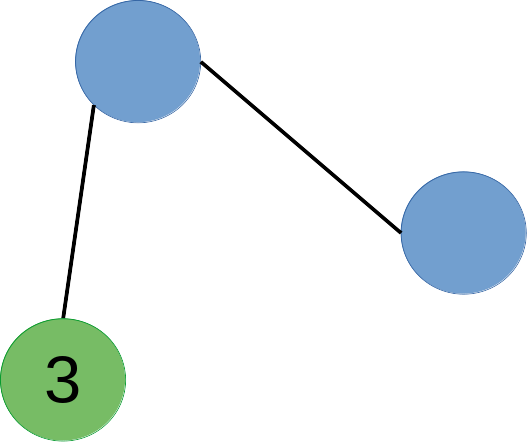
\includegraphics[width=0.2\textwidth]{simplex_2.png}
                    \caption{Three nodes from the left image united in 3-simplex having properties of the initial vertices}
                \end{multicols}
            \end{figure}
    \end{itemize}

